\chapter{Decision Making}

An AI agent should be capable of making decisions. Based on what it observes, what it believes, and what it desires, the agent must determine the most beneficial action or sequence of actions to take. In many practical problems, the consequences of actions or even the “best” reachable states of the system are not known in advance. The AI agent must therefore rely on trial and error, learning from successful and failed attempts to develop an optimal policy across different scenarios.

This chapter studies several models of decision making. Among them, the Markov Decision Process is discussed in detail, as it is one of the most widely used decision-making frameworks.

\section{Utility}

To formulate a decision-making problem mathematically, the first step is to define the \mync{utility} (often in the form of a function) that quantifies the value of an action or system state. Decision making is essentially the process of maximizing utility. This section introduces the concept of utility and the formulation of utility functions.

\subsection{Utility Theory}

Intuitively, a rational AI agent should always choose the action that maximizes expected utility among all available actions. This is known as the \mync{maximum expected utility} (MEU) principle. Below, MEU is formulated as an optimization problem.

When an action is taken, the system transitions from one state to another. Let the transition model be denoted by $P(s|a,e)$, where $e$ represents the evidence or observation of the system, incorporating the agent’s awareness of its current state; $a$ denotes the action taken; and $s$ is the resulting state. The probabilistic form of $P(s|a,e)$ captures uncertainty in the system.

Upon reaching state $s$, a utility $U(s)$ is obtained. The utility $U(s)$ usually includes not only the immediate benefit of being in $s$ but also the foreseeable future benefits that may arise from reaching $s$ as an intermediate state.  

The expected utility of an action $a$, given evidence $e$, over possible landing states $s_i \in S$, is expressed as
\begin{eqnarray}
	EU(a|e) &=& \sum_{s_i \in S} P(s_i|a,e) U(s_i) \label{eq:expected_utility}
\end{eqnarray}

Given the evidence $e$, an AI agent may take one of several actions $a_i \in A$. MEU suggests that the optimal action is
\begin{eqnarray}
	a^* &=& \argmax_{a_i \in A} EU(a_i|e) \label{eq:emu}
\end{eqnarray}

An example of MEU is shown in Fig.~\ref{fig:emuexp}. Consider a maze in which the AI agent is randomly placed in one of several locations (blocks). Each location corresponds to a state. The agent can move horizontally or vertically one step at a time. The distance from each block to the “GOAL” represents the utility of that state.

\begin{figure}[!htb]
	\centering
	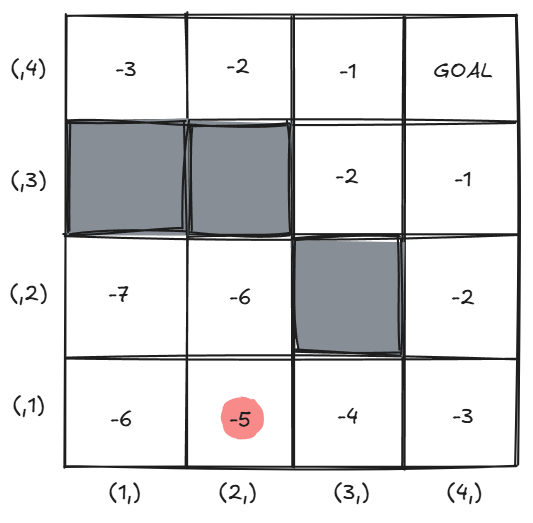
\includegraphics[width=0.5\textwidth]{./chapters/part-1/figures/emuexp.png}
	\caption{State utility map in the MEU example.}
	\label{fig:emuexp}
\end{figure}

Let $e$ represent the agent’s current location, assumed to be the red dot at $(2,1)$. The agent can take four actions, listed below along with their possible resulting states and associated probabilities:
\begin{eqnarray}
	a_1 &=& \mathrm{UP} \nonumber \\
	P((2,1)|a_1,e) &=& 0.2 \nonumber \\
	P((2,2)|a_1,e) &=& 0.6 \nonumber \\
	P((1,1)|a_1,e) &=& 0.1 \nonumber \\
	P((3,1)|a_1,e) &=& 0.1 \nonumber \\
	a_2 &=& \mathrm{LEFT} \nonumber \\
	P((2,1)|a_2,e) &=& 0.2 \nonumber \\
	P((2,2)|a_2,e) &=& 0.1 \nonumber \\
	P((1,1)|a_2,e) &=& 0.6 \nonumber \\
	P((3,1)|a_2,e) &=& 0.1 \nonumber \\
	a_3 &=& \mathrm{DOWN} \nonumber \\
	P((2,1)|a_3,e) &=& 0.7 \nonumber \\
	P((2,2)|a_3,e) &=& 0.1 \nonumber \\
	P((1,1)|a_3,e) &=& 0.1 \nonumber \\
	P((3,1)|a_3,e) &=& 0.1 \nonumber \\
	a_4 &=& \mathrm{RIGHT} \nonumber \\
	P((2,1)|a_4,e) &=& 0.2 \nonumber \\
	P((2,2)|a_4,e) &=& 0.1 \nonumber \\
	P((1,1)|a_4,e) &=& 0.1 \nonumber \\
	P((3,1)|a_4,e) &=& 0.6 \nonumber
\end{eqnarray}

Note that the outcome of an action is not deterministic. In practice, this may result from signal transmission errors or environmental uncertainty. The agent cannot move downward from its current location, so when it chooses the “DOWN” action $a_3$, it will likely remain in the same place after encountering a wall.

Using \eqref{eq:expected_utility}, the expected utility of $a_1$ can be computed as
\begin{eqnarray}
	EU(a_1|e) &=& 0.2 \times (-5) + 0.6 \times (-6) + 0.1 \times (-6) + 0.1 \times (-4) \nonumber \\
	&=& -5.6 \nonumber
\end{eqnarray}
Similarly, $EU(a_2|e) = -5.6$, $EU(a_3|e) = -5.1$, and $EU(a_4|e) = -4.6$. Therefore, according to \eqref{eq:emu}, the rational decision is to take action $a_4$, i.e., move “RIGHT.”

In this example, all states $s_i$, transition probabilities $P(s_i|a,e)$, and utilities $U(s_i)$ are assumed known. This is rarely the case in practical problems. Sections~\ref{sec:mdp} and~\ref{sec:pomdp} will introduce methods for estimating or learning these quantities.

\begin{mdframed}
	\noindent \textbf{Are there alternatives to expected utility?}
	
	The expected utility of an action is calculated using \eqref{eq:expected_utility}. An AI agent using \eqref{eq:expected_utility} and \eqref{eq:emu} to make decisions behaves rationally. 
	
	However, can we base decision making on other measures of utility? For example, consider the worst-case utility:
	\begin{eqnarray}
		WU(a|e) &=& \min\{U(s_i)\,|\,P(s_i|a,e) > 0\} \nonumber
	\end{eqnarray}
	Instead of maximizing expected utility, could we maximize worst-case utility?
	
	This question concerns the definition of a rational agent. To formalize this, the following \mync{axioms of utility theory} are defined:
	\begin{itemize}
		\item \textbf{Orderability.} For any two actions $a_1$ and $a_2$, exactly one of the following statements must hold: “$a_1$ is preferred over $a_2$,” “$a_1$ and $a_2$ are indifferent,” or “$a_2$ is preferred over $a_1$.” Thus, any two actions can be ranked.
		\item \textbf{Transitivity.} If $a_1$ is preferred over $a_2$ and $a_2$ is preferred over $a_3$, then $a_1$ must be preferred over $a_3$.
		\item \textbf{Continuity.} For three actions $a_1$, $a_2$, and $a_3$, where $a_1$ is preferred over $a_2$ and $a_2$ over $a_3$, there exists a probability $p$ such that a compound action $a_{1,3,p,1-p}$ (which randomly chooses $a_1$ with probability $p$ and $a_3$ with $1-p$) is indifferent to $a_2$.
		\item \textbf{Substitutability.} If $a_1$ and $a_2$ are indifferent and $a_3$ is any action, then for any $p$, the compound actions $a_{1,3,p,1-p}$ and $a_{2,3,p,1-p}$ must be indifferent.
		\item \textbf{Monotonicity.} If $a_1$ is preferred over $a_2$, then for compound actions $a_{1,2,p_1,1-p_1}$ and $a_{1,2,p_2,1-p_2}$, if $p_1 > p_2$, then $a_{1,2,p_1,1-p_1}$ is preferred over $a_{1,2,p_2,1-p_2}$.
		\item \textbf{Decomposability.} Compound actions can be nested or decomposed. For example, if $a_{1,2,p,1-p}$ is a compound action and $a_2$ is itself a compound action $a_2 = a_{21,22,q,1-q}$, then $a_{1,2,p,1-p}$ is indifferent to $a_{1,21,22,p,(1-p)q,(1-p)(1-q)}$.
	\end{itemize}
	
	Let $U(a|e)$ (or simply $U(a)$) denote the utility of action $a$. The specific form of $U(a)$, whether it represents expected utility or another valid measure, is acceptable as long as the following conditions are satisfied:
	\begin{itemize}
		\item $U(a)$ must exist for every action.
		\item $U(a)$ must reflect preference: if $U(a_1) > U(a_2)$, then $a_1$ is preferred over $a_2$; if $U(a_1) = U(a_2)$, they are indifferent.
		\item The preferences reflected by $U(a)$ satisfy the axioms of utility theory.
	\end{itemize}
	
	For any utility $U(a)$ satisfying these criteria, the utility of a compound action composed of actions $a_1, \dots, a_n$ with corresponding probabilities $p_1, \dots, p_n$ is given by
	\begin{eqnarray}
		U(a_{1,2,\dots,n,p_1,p_2,\dots,p_n}) &=& \sum_i p_i U(a_i) \nonumber
	\end{eqnarray}
	
	Note that the utility function is not unique. For instance, given a utility function $U(a)$,
	\begin{eqnarray}
		U'(a) &=& \alpha U(a) + \beta, \quad \alpha > 0 \nonumber
	\end{eqnarray}
	is also a valid utility function.
	
\end{mdframed}

\subsection{Utility Function}

The utility of an action $U(a|e)$, for example $EU(a|e)$ as in \eqref{eq:expected_utility}, is an instance of a \mync{utility function} that maps actions to real numbers. As noted earlier, the expected utility formulation is not the only valid approach consistent with the axioms of utility theory. Nonetheless, it is the most widely used and is employed in the \myabb{Markov Decision Process}{MDP}, which will be introduced in Sections~\ref{sec:mdp} and~\ref{sec:pomdp}. For the remainder of this chapter, unless otherwise specified, we consider expected utility as defined in \eqref{eq:expected_utility}.

The expected utility of an action depends on the transition model $P(s|a,e)$ and the state utility $U(s)$. State utility typically includes both its immediate reward and the anticipated future utility obtainable from using that state as an intermediate step. For example, in chess, each board configuration represents a state. Only the final checkmate state provides immediate utility, but intermediate states possess utility as they contribute to eventual victory.

The computation of utility functions for actions and states is often referred to as \mync{preference elicitation}. Different models have different ways of defining and calibrating utility functions. As far as this notebook concerns, utility calculation of MDP will be introduced in details in Sections~\ref{sec:mdp} and \ref{sec:pomdp}. In the remainder of this section, factors and good practices of determine utilities, especially immediate reward of a state, are discussed. Notice that anticipated future utilities of states and utilities of actions can often be derived from the immediate rewards of states and the transition models.

While the detailed calculation of utilities varies by task and will be addressed later, some general principles for assigning utility values are useful and they are given below.
\begin{itemize}
	\item Although utility is relative, it is often helpful to define global upper and lower bounds, where the lower bound represents “immediate loss” and the upper bound represents “goal achieved.”
	\item In many real-world problems, utility is expressed in monetary terms (financial gain or cost). Rewards and penalties of various types are converted to monetary values and normalized by a scaling factor.
	\item Decision makers may differ in risk preference. Risk-averse and risk-seeking agents can have different utility functions even under identical circumstances.
	\item Mathematically derived utility functions sometimes contradict human intuition, as humans are not always rational and do not always conform to the axioms of utility theory.
\end{itemize}

An \mync{influence diagram} or \mync{decision network} represents the structure of a utility function. It is a graphical model illustrating the relationships between utility, its contributing attributes, and the factors influencing those attributes, as well as the entities responsible for making decisions. Understanding this structure helps decision makers identify which factors influence outcomes and should be considered when determine the utility values.

An example is shown in Fig.~\ref{fig:decisionnetworkexp}, where a decision network assists a buyer in choosing a house. Here, the utility function depends on three attributes—location, construction quality, and price—each determined by several underlying factors. The entity ``buyer'' controls these attributes, selecting actions (purchase choices) that maximize utility.

\begin{figure}[!htb]
	\centering
	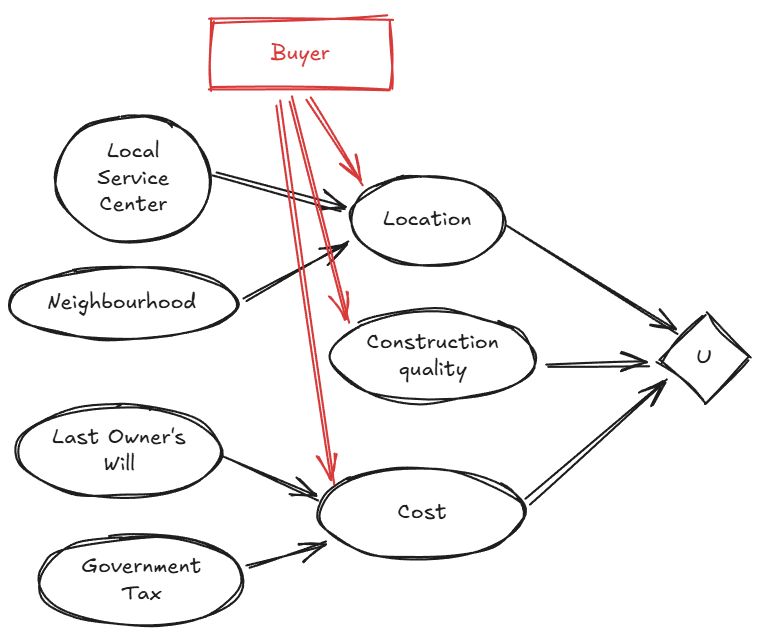
\includegraphics[width=0.75\textwidth]{./chapters/part-1/figures/decision_network_exp.png}
	\caption{A simple decision network in which a buyer must decide which house to purchase.}
	\label{fig:decisionnetworkexp}
\end{figure}

\section{Markov Decision Process} \label{sec:mdp}

Till this point, the basic principle of decision making has been introduced. In a nutshell, utilities (or utility functions) need to be defined for each action. The utility function should be designed to fulfill the axioms of utility theory so that the agent will behave rationally. The decision map helps with formulating the utility function. The action with the highest expected utility should be chosen, which is known as MEU. 

An example has been given where the utility is determined by \eqref{eq:expected_utility} and MEU is realized by \eqref{eq:emu}. We have briefly mentioned that the formulation of utility function is not unique and different formulation methods may have different ways to calibrate utility values. 

In this and the following up sections, MDP is introduced. MDP is probably one of the most widely used way of formulating the decision making problem. In fact, the formulation demonstrated by \eqref{eq:expected_utility} is a subclass of MDP.

\subsection{Formulation}

\mync{Markov Decision Process}[MDP] refers to the following decision making problem formulation. 
\begin{itemize}
	\item It defines ``state'', which is a minimum set of information that reflects the current status of the system.
	\item It defines ``transition model'', which is a description of the relationship of current state, action to take, and the resulted new state by the action. The transition model is often given by stochastic model $P(s\textprime|s,a)$ (essentially the same with $P(s|a,e)$ in \eqref{eq:expected_utility} where the current state information is given in evidence $e$). The transition model is Markovian, i.e., it concerns only the current but not historical states and actions.
	\item The decision is made in sequence, i.e., it makes decision, transforms states, and make another decision, and transform states again, until certain termination condition is reached.
	\item A utility function is defined for the agent. The utility depends on a sequence of states that the agent has reached. When transforms into a state, the agent gains some reward $R(s)$ (can be positive, zero or negative).
\end{itemize}

To implement MDP, there are at least the following two challenges.
\begin{itemize}
	\item The utility of each state, $U(s_i)$, is often not obvious, and needs to be calculated by searching or learning.
	
	In some scenarios, we are not aware what is the best achievable state. Consider the example in Fig.~\ref{fig:emuexp} where the map is much larger and the goal is hidden. The agent would know the goal only when it reaches there and get a very high reward. Yet, it does not know whether that large reward comes from the global optimum goal or just a local optimum.
	
	\item The probabilities $P(s|a_i,e)$ needs to be calibrated.
	
	In some scenarios, we know the goal state that we want to reach out to, but we are not aware of what action or actions sequence can lead us to that state. Consider the example in Fig.~\ref{fig:emuexp}. Assume that the four actions are not named ``UP'', ``LEFT'', ``DOWN'' and ``RIGHT'', but simply ``A'', ``B'', ``C'' and ``D''. To make it even more complicated, assume that at each state, i.e., when the agent is at different locations, the correlation of the four bottoms to the agent movement varies.
	
\end{itemize}

Assume that all the probable states, all the transaction models (including actions and stochastic models) and all the rewards are known prior to a decision making. In this MDP formulation, the system is fully observable. The purpose of the MDP is to decide the action at each state that maximizes the agent utility when the terminate condition is fulfilled. This optimal action at each state is known as the \mync{optimal policy} of MDP, often denoted by
\begin{eqnarray}
	\pi^*: s \rightarrow a \nonumber
\end{eqnarray}
For example, the optimal policy for the example in Fig.~\ref{fig:emuexp} is given by Fig.~\ref{fig:emuexppistar}
\begin{figure}[!htb]
	\centering
	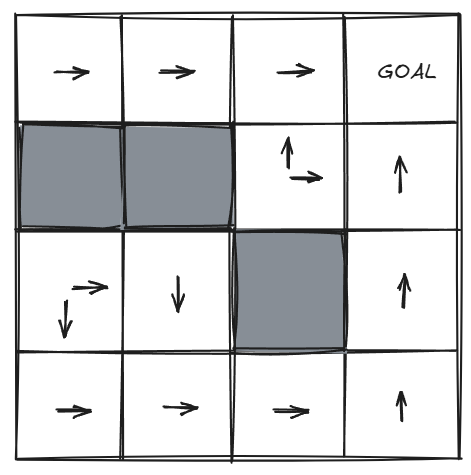
\includegraphics[width=0.5\textwidth]{./chapters/part-1/figures/emuexppistar.png}
	\caption{State utility map for in the MEU example.}
	\label{fig:emuexppistar}
\end{figure}

The study of MDP focuses on finding out $\pi^*$ in a systematical manner. Notice that this section assumes fully observable MDP, while the next Section~\ref{sec:pomdp} studies \myabb{Partially Observable MDP}{POMDP} where the transition model and rewards may not be known from the start.

Depending on whether there is a finite horizon, MDP can be divided into the following categories.
\begin{itemize}
	\item Finite horizon. There is a fixed horizon $N$. After $N$ actions, the game is over and nothing matters beyond that horizon, and no more utility will be counted. The purpose is to gain as much utility as possible within $N$ actions.
	
	Notice that in this case, the optimal policy is non-stationary and may vary depending on the remaining time. Assume that for some reason the agent circles back to the same state after $k<N$ actions. The optimal policy by then, with only $N-k$ actions remaining, might be different from when the agent had $N$ actions remaining.
	
	\item Infinite horizon. The game does not have a time limit and the agent is allowed to recurrently take actions and transform states forever.
	
	Notice that in this case, the optimal policy is stationary. The optimal action at a state is fixed and not affected by the timestamp when the agent reaches that state. Several ``terminating states'' can be defined, where when the agent reaches those states, the game ends. Those terminating states is often assigned with very large rewards (mission completed) or penalties (mission failed).
\end{itemize}

As introduced earlier, the utility function of an agent depends on the state the agent has visited. When deciding the optimal policy, it is often assumed that the agent's preferences between state sequences are stationary, meaning that given a fixed starting state (and a fixed horizon, if it is a finite horizon problem), the agent always plans to take the same (sequence of) actions. With that assumption, there is only one way to formulate the utility function, namely the \mync{discounted rewards utility function} given by
\begin{eqnarray}
	U(s_0, s_1, s_2, \ldots) &=& R(s_0) + \gamma R(s_1) + \gamma^2R(s_2) + \ldots \label{eq:discountedreward}
\end{eqnarray}
where $s_i$ are the states an agent visits in sequence, and $0 < \gamma \leq 1$ the discount factor. In the special case where $\gamma = 1$, the discounted rewards utility function reduces to \mync{additive rewards utility function}.
For now, simply assume that $R(s_i)$ in \eqref{eq:discountedreward} is pre-assigned for each state. As will be introduced in next sections, there are ways to calibrate the reward at each state.

\begin{mdframed}
\noindent \textbf{Is agent utility always bounded?}

From \eqref{eq:discountedreward}, in an infinite horizon MDP formulation the utility is not necessarily bounded. For example, consider a robot agent moving inside a maze with infinite horizon. If there are two states $s_1$ and $s_2$, both adding positive utilities to the agent, the agent may choose to move in between these two states indefinitely to gain infinite utility, and it will never targeting on finding the goal, even if an extremely large utility is assigned to the goal state. In this case, MDP fails and it cannot generate rational decisions.

When agent utility is unbounded, MDP will fail to make rational decisions.

To ensure that MDP is bounded, and to encourage it to get rid of loops and find the ``goal`` as soon as possible, consider the following approaches.
\begin{itemize}
	\item Use discounted rewards with $\gamma < 1$. This guarantees that the agent utility is bounded and encourages MDP to reach the state with the highest utility as soon as possible.
	\item Assign small negative rewards for all ``intermediate'' states to encourage MDP to not waste time wondering around. 
\end{itemize}

It is recommended to use both or at least the first approach to ensure that utility is bounded.

\end{mdframed}




















The utility of a state can be taken as an extension to the utility of an action. For example, in \eqref{eq:expected_utility} the utility of a state $U(s)$ is often calculated as the maximum value of utility functions among all probable actions on that state, i.e.,
\begin{eqnarray}
	U(s) &=& \max_i \left(EU(a_i|e)\right) \label{eq:stateutility}
\end{eqnarray}
where $a_i$ is any probable action that can be taken at state $s$. Using \eqref{eq:stateutility}, the utility of states can be calculated from the utility of actions.

The calculation of utility functions can be challenging. For example, consider $U(a|e)$ given by \eqref{eq:expected_utility}. The transaction probability $P(s|a,e)$ and the state utility $U(s)$ are usually unknown in the beginning and need to be calibrated. There are different ways to calibrate their values. In the later Sections \ref{sec:mdp} and \ref{sec:pomdp}, the calculation of utility functions in Markov decision process, one of the most widely used decision making model, will be introduced in more details.

\subsection{Value Iteration}

Bellman equation and convergence.

\subsection{Policy Iteration}

\section{Partially Observable MDP} \label{sec:pomdp}

\mync{Partially Observable Markov Decision Process}[POMDP] refers to ...

\section{Multi-attribute Utility Function}

To this point, we have been assuming that all the attributes that affect utility can converted and put on the same scale. When maximizing the utility, only that single figure is considered. However, this is not always true in the reality. For example, consider personal protective equipment design. In practice, there is always a chance that the protection fails. It will take infinite money to make the equipment infinitely safe. To maximize the utility, we need to put financial cost and human life on the same scale, which is difficult and can be immoral.

A problem whose outcomes are characterized by two or more attributes that cannot be easily converted into a single figure are handled by \mync{multi-attribute utility theory}. There are several ways to handle the situation, and they are briefly introduced as follows.

In the heat map approach, the actions are converted into coordinates in a hyper space where each dimension representing an attribute. A heat map is constricted, representing the safe and dangerous zones in the hyper space. Actions inside the safe zone are selected.

In the statistic dominance approach, we investigate the chance that an action may perform better than any other actions in every aspects. The action that statistically more likely to dominant (perform better than other actions in all attributes) is selected.

Sometimes the attributes follow joint distribution. We can set a lower bound for one of the attributes, hence reducing the problem to a single-attribute problem. That attribute is used to formulate the utility function. Consider the earlier personal protective equipment example. The more expensive the gear, the more likely it is safe. The safety and the cost form a positively correlated joint distribution, where each sample in the distribution is an action. We can set a lower bound for safety requirements, for example, safety probability of $99.999\%$, and reduce the problem to a single attribute problem where we find the action with the minimum financial cost that guarantees the safety probability.

\section{Game Theory}

Multi-agent control system.